\documentclass[11pt, oneside]{article}   	% use "amsart" instead of "article" for AMSLaTeX format
\usepackage{geometry}                		% See geometry.pdf to learn the layout options. There are lots.
\geometry{letterpaper}                   		% ... or a4paper or a5paper or ... 
\usepackage[parfill]{parskip}    			% Activate to begin paragraphs with an empty line rather than an indent
\usepackage{graphicx}				% Use pdf, png, jpg, or eps� with pdflatex; use eps in DVI mode
								% TeX will automatically convert eps --> pdf in pdflatex		
\usepackage{amssymb}

\usepackage{algorithm}
\usepackage{algorithmic}

\usepackage{listings}
\usepackage{color}
\definecolor{dkgreen}{rgb}{0,0.6,0}
\definecolor{gray}{rgb}{0.5,0.5,0.5}
\definecolor{mauve}{rgb}{0.58,0,0.82}

\lstset{frame=tlrb,
  language=C++,
%  aboveskip=3mm,
% belowskip=3mm,
  showstringspaces=false,
  columns=flexible,
  basicstyle={\small\ttfamily},
  numbers=none,
  numberstyle=\tiny\color{gray},
  keywordstyle=\color{blue},
  commentstyle=\color{dkgreen},
  stringstyle=\color{mauve},
  breaklines=true,
  breakatwhitespace=true
  tabsize=3
}
\title{A Quick Tutorial on Using the GenericIO Reader}

\begin{document}
\maketitle

This document provides a quick tutorial on how to link the GenericIO library and use the GenericIO reader
within a C/C++ application. It is assumed that the reader has downloaded and compiled the source based on 
the instructions in the supplied {\tt README} file.

\section{Linking to the GenericIO library}
GenericIO is compiled as a static library. It is assumed that the code is installed in
a directory {\tt <GIOROOT>} and compiled by running {\tt `make`} within the
root directory. A C/C++ executable, e.g., {\tt mymain.cxx}, can then be compiled and link to the library
by adding the following to the {\tt Makefile} (or by just running the corresponding command in a terminal).
\begin{lstlisting}
FLAGS=-I<GIOROOT>
LDFLAGS=-L<GIOROOT>/genericio.build/libs -lGenericIO

all:
 mpicxx  ${FLAGS} -o mymain mymain.cxx ${LDFLAGS}
\end{lstlisting}

This should be adapted for the target platform, e.g., use {\tt CC} if you are compiling on a Cray or {\tt mpixlcxx\_r} if
you are compiling on a BlueGene. Note, although the client application may be coded in {\tt C}, a {\tt C++} compiler 
must be used since the GenericIO library is a {\tt C++} code.
\newpage

\section{Using the GenericIO Reader}
\label{section:basic}
Using the GenericIO reader within an application can be achieved in the following steps:
\begin{enumerate}

\item Add include directives for the GenericIO library as illustrated below:
\begin{lstlisting}
// GenericIO includes
#include "GenericIODefinitions.hpp"
#include "GenericIOReader.h"
#include "GenericIOMPIReader.h"
#include "GenericIOPosixReader.h" 
\end{lstlisting}

\item Allocate the reader object. The GenericIO library provides two modes of parallel I/O: (a) using the POSIX
library and (b) using MPI I/O. Applications can then allow the user to select the desired underlying method 
for I/O, i.e., via a command line argument, and then allocate the appropriate GenericIO reader as demonstrated
in the code snippet below:
\begin{lstlisting}
// Allocate GenericIOReader Object
gio::GenericIOReader* reader = NULL;
if( usePosix ) {
  reader = new gio::GenericIOPosixReader();
}
else {
  reader = new gio::GenericIOMPIReader();
}
\end{lstlisting} 

\item Setup the reader parameters. Namely, specify the filename and path of the file to open and register the
underlying {\tt MPI} communicator for this operation.
\begin{lstlisting}
reader->SetFileName( fileToRead );
reader->SetCommunicator( comm );
\end{lstlisting}

\item Next, the application must read the header metadata. This is done in a collective call, hence all MPI ranks
must call the following method.
\begin{lstlisting}
// This is a collective call. All ranks must call this!
reader->OpenAndReadHeader();
\end{lstlisting}

\item Once the header is read, each process can obtain the number of elements, $N$, it will read by the following call:
\begin{lstlisting}
int N = reader->GetNumberOfElements();
\end{lstlisting}

\item Then, $N$  is used to allocate the application arrays wherein the data from the file will be stored. 
Once the application arrays are allocated, they are registered in the reader with the corresponding
variable  name from the file.
Note, that this requires knowing {\em a priori} the name of the variables to read in and the corresponding primitive type, e.g., 
{\tt float}, {\tt int}, etc. To facilitate with this, the GenericIO library provides the {\tt GenericIOInspector} utility, which
can be run on the file to retrieve the required information -- run "{\tt ./GenericIOInspector --help}" for the details on
how to use it and look at the supplied {\tt README} for more details. To illustrate this step, the code snippet below 
reads the $x,y,z$ coordinates from a HACC particle dataset.
\begin{lstlisting}
N = reader->GetNumberOfElements();

// Get padsize for floats
int floatpadsize = gio::CRCSize/sizeof(float);

// Allocate application arrays to store variables in this rank.
// NOTE: arrays are padded to have sufficient space to store 
// the Cyclic-Redundancy-Check (CRC), used to validate the data. 
// This is done such that the data and the CRC will be read in with a 
// single read, that way minimizing the I/O overhead.
float* x = new float[ N+floatpadsize ];
float* y = new float[ N+floatpadsize ];
float* z = new float[ N+floatpadsize ];

// Register application arrays with the reader, corresponding
// to the variable being read
reader->AddVariable("x", x, gio::GenericIOBase::ValueHasExtraSpace);
reader->AddVariable("y", y, gio::GenericIOBase::ValueHasExtraSpace);
reader->AddVariable("z", z, gio::GenericIOBase::ValueHasExtraSpace);
\end{lstlisting}

\item Last, the data is read in to the supplied arrays by the following collective call.
\begin{lstlisting}
// This is a collective call. All ranks must call this!
reader->ReadData();
\end{lstlisting}
\end{enumerate}

%%
\section{Block Redistribution}
The data in GenericIO is written in blocks. Each block in the file corresponds to the MPI rank that wrote the data 
(i.e., the rank from HACC). However, an application may read in the data using a different number of ranks. 
Consider an application with {\tt NRANKS} reading a file with {\tt NBLOCKS}. The three possible scenarios
and corresponding behavior of the GenericIO reader are summarized in Table~\ref{distribution}.
\begin{table}[h!]
\caption{ \label{distribution} Summary of Block Distribution Scenarios \& Handling in the GenericIO Reader }
\centering
\begin{tabular}{|c | l |} \hline\hline
{\bf Scenario}				    & {\bf GenericIO Reader Behavior} \\\hline
{\tt NRANKS} == {\tt NBLOCKS}   & Blocks are mapped to processes one-to-one \\\hline
{\tt NRANKS} $>$ {\tt NBLOCKS} & Block $b_i$ is assigned to process $P_i$, $P_j$ has no data $\forall j \ge$ {\tt NBLOCKS} \\\hline
{\tt NRANKS} $<$ {\tt NBLOCKS} & Round-Robin (default) or RCB assignment (spatially contiguous) \\\hline	
\end{tabular}
\end{table}

The last scenario, where {\tt NRANKS} $<$ {\tt NBLOCKS}  turns out to be quite common. 
The approach outlined in Section~\ref{section:basic} will work transparently. From the application/developer 
perspective the data is read into a single array buffer. However, internally the reader will fuse the blocks into
the user-supplied buffer.  By default the GenericIO reader will use round-robin assignment of blocks 
to the application processes. Depending on the application, this may be sufficient, but will result in
spatially disjoint regions of data. 

Most often, it is desirable to read in the data in spatially contiguous chunks.
HACC uses an MPI cartesian communicator for its decomposition. Each rank
is associated with an $(i,j,k)$ coordinate, which is available in the block headers
in the GenericIO data. For these outputs, the reader provides an additional block
assignment strategy, which is based on Recursive Coordinate Bisection (RCB), that
can produce spatial contiguous chunks of data for each rank. To use this assignment
strategy, amount to one additional call when setting up the reader parameters as 
illustrated below. 
\begin{lstlisting}
reader->SetFileName( fileToRead );
reader->SetCommunicator( comm );
// Override the default Round-Robin assignment strategy and use RCB
reader->SetBlockAssignmentStrategy( gio::RCB_BLOCK_ASSIGNMENT );
\end{lstlisting}

Note, the call to {\tt SetBlockAssigmentStrategy} must be prior 
to calling {\tt OpenAndReadHeader}. Figure~\ref{figures} depicts the differences of
reading the data using round-robin and RCB.
\begin{figure}[h!]
\centering
$\begin{array}{c c}
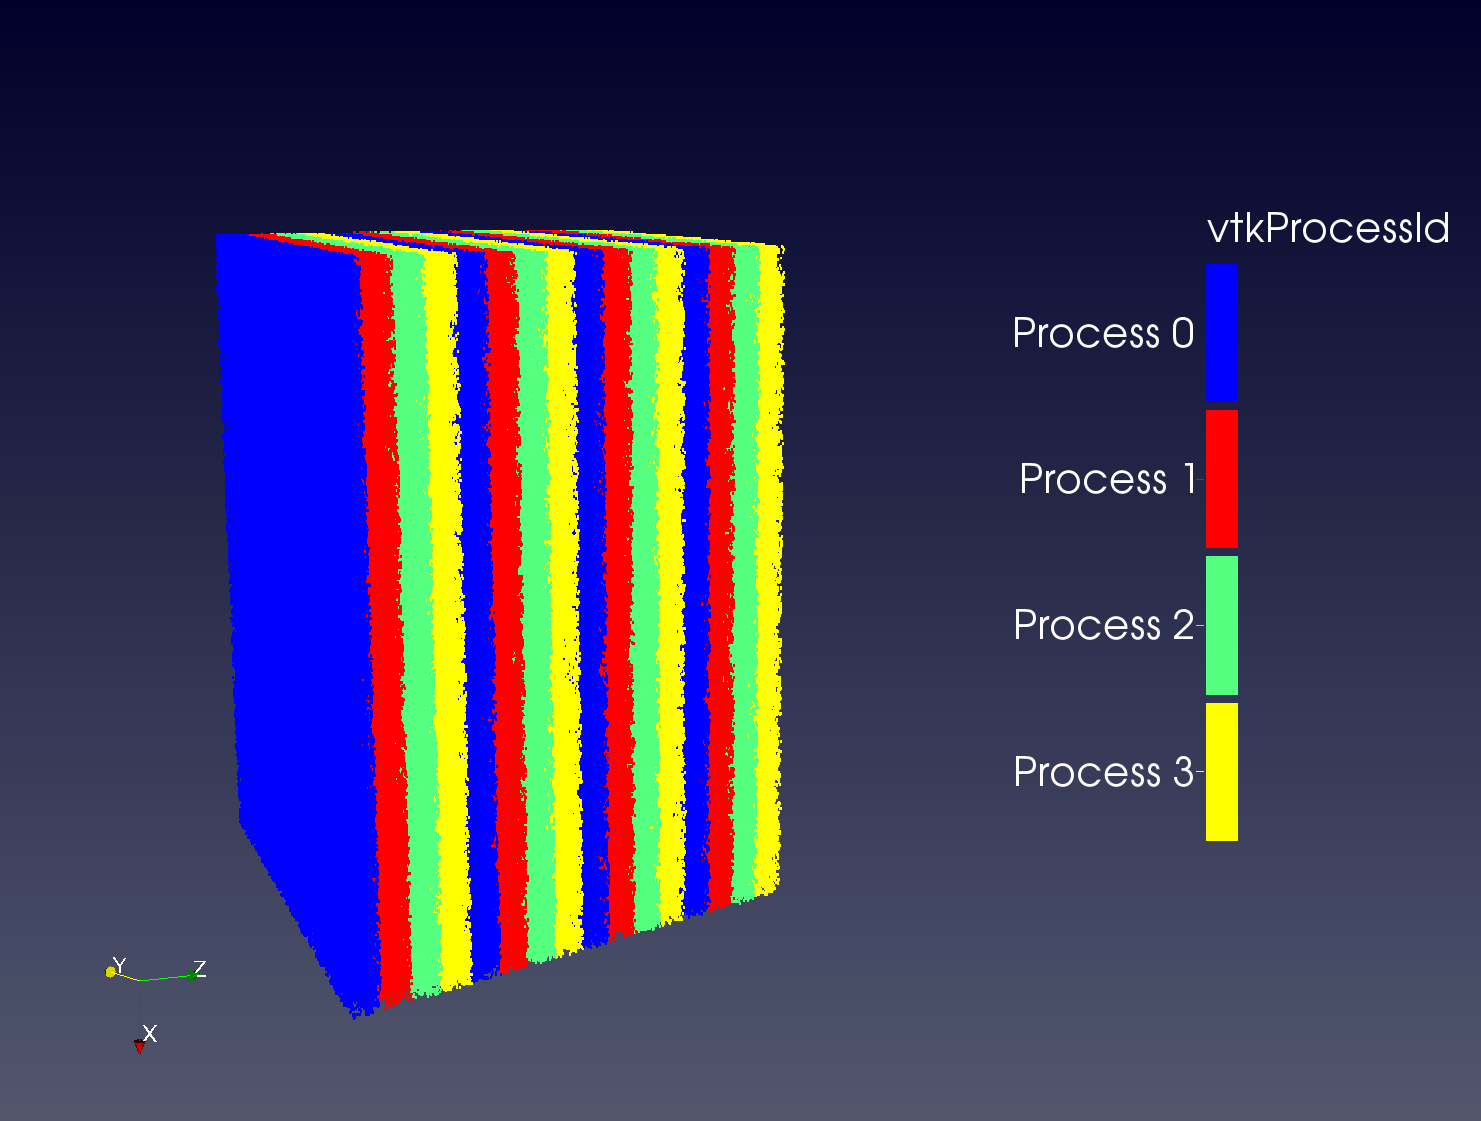
\includegraphics[width=3in]{figures/GIORoundRobin.png} &
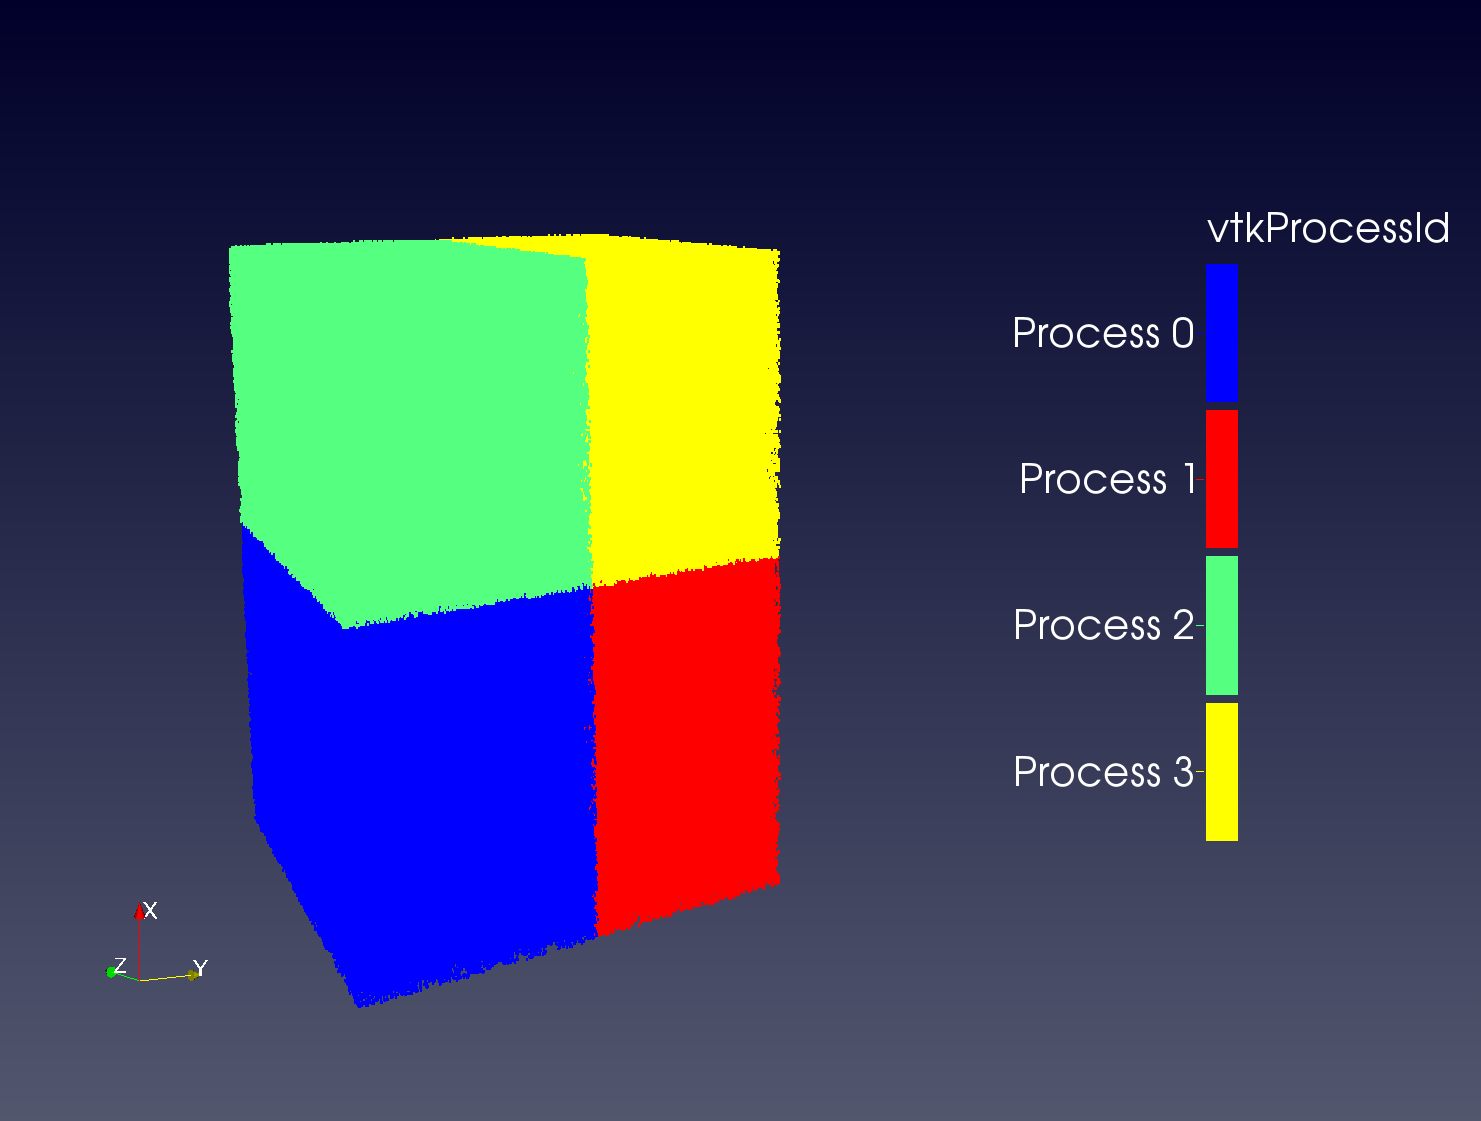
\includegraphics[width=3in]{figures/GIORCB.png} \\
(a) & (b)
\end{array}$
\caption{ \label{figures} Round-Robin(left) Vs. RCB Assignment(right). }
\end{figure}

\subsection{Acquire Neighboring Rank Topology}
While reading the data in spatially contiguous chunks, using the RCB assignment,  
solves several issues, applications often require to communicate with neighbors to
carry out certain tasks/computations. Again by exploiting the fact that HACC uses
an MPI cartesian communicator, the GenericIO reader provides a mechanism to
query the neighbors of each process.
\newpage
The data-structure to store neighbors stores the neighboring rank and an orientation
tuple with respect to the given process as shown below:
\begin{lstlisting}
struct RankNeighbor {
  int RankID;	   // neighboring rank ID
  int Orient[3];   // orientation of the neighbor w.r.t. this process
};
\end{lstlisting}

The orientation tuple stores the neighboring relationship of the given process and the neighboring
rank along each dimension. The list of possible values are given by an enum, called {\em NeighborOrientation},
shown below:
\begin{lstlisting}
enum NeighborOrientation {
   ON_MIN,              	//!< neighbor is abutting at the min end
   ON_MAX,              	//!< neighbor is abutting at the max end
   OVERLAPPING,    		//!< neighbor extents are overlapping
   ON_MAX_MIN_PERIODIC, 	//!< neighbor is abutting on the max end and along
             			//!< the min periodic boundary.
   ON_MIN_MAX_PERIODIC, 	//!< neighbor is abutting on the min end and along
                        	//!< the max periodic boundary.
   MIN_PERIODIC,        	//!< abutting along the min periodic boundary
   MAX_PERIODIC,        	//!< abutting along the max periodic boundary
   NOT_CONNECTED,      		//!< neighbor is not connected
   UNDEFINED,           	//!< neighbor relationship has not been defined
 };\end{lstlisting}

An application can utilize the neighbor orientation to decide what data should be communicated and
whether a transform should be applied. For example, if a neighbor is abutting on the right, the orientation
tuple, would be {\tt \{ON\_MAX,OVERLAPPING,OVERLAPPING\}}. The process would then exchange
the data on its right boundary with the given neighbor. A different process, may have a neighbor across
the left periodic boundary. For example, in this case the orientation tuple would be 
{\tt \{MIN\_PERIODIC,OVERLAPPING,OVERLAPPING\}}. The process would then have to exchange the
data on its left boundary, however, the data may need to be transformed before or after communication 
takes place to account for periodicity.

Neighbors can be queried after the call to {\tt OpenAndReadHeader} using the following
code:
\begin{lstlisting}
// Allocate vector to store neighbors
std::vector< gio::RankNeighbor > neighbors;
neighbors.resize( reader->GetNumberOfRankNeighbors() );

// Get the neighbors
reader->GetRankNeighbors( &neighbors[0] );
\end{lstlisting}

It should be noted that neighbor information is only available if reading the data using RCB assignment.
For completeness, the next section provides complete code for a sample application.
\newpage

\section{Sample Application}

\begin{lstlisting}
// GenericIO includes
#include "GenericIODefinitions.hpp"
#include "GenericIOReader.h"
#include "GenericIOMPIReader.h"
#include "GenericIOPosixReader.h"
// MPI include
#include <mpi.h>
int main(int argc, char** argv)
{
  MPI_Init(&argc,&argv);
  MPI_Comm comm = MPI_COMM_WORLD;
  
  // Allocate GenericIOReader Object
  gio::GenericIOReader* reader = NULL;
  if( usePosix ) {
    reader = new gio::GenericIOPosixReader();
  }
  else {
    reader = new gio::GenericIOMPIReader();
  }
  
  // Set reader parameters
  reader->SetFileName( fileToRead );
  reader->SetCommunicator( comm );
  // Use RCB block distribution to read in blocks in spatially contiguous
  if( useRCB )
    reader->SetBlockAssignmentStrategy(gio::RCB_BLOCK_ASSIGNMENT);
    
  // This is a collective call. All ranks must call this!  
  reader->OpenAndReadHeader();
  
  N = reader->GetNumberOfElements();
  
  // Get padsize for floats
  int floatpadsize = gio::CRCSize/sizeof(float);

  // Allocate application arrays to store variables in this rank.
  // NOTE: arrays are padded to have sufficient space to store 
  // the Cyclic-Redundancy-Check (CRC), used to validate the data. 
  // This is done such that the data and the CRC will be read in with a 
  // single read, that way minimizing the I/O overhead.
  float* x = new float[ N+floatpadsize ];
  float* y = new float[ N+floatpadsize ];
  float* z = new float[ N+floatpadsize ];

  // Register application arrays with the reader, corresponding
  // to the variable being read
  reader->AddVariable("x", x, gio::GenericIOBase::ValueHasExtraSpace);
  reader->AddVariable("y", y, gio::GenericIOBase::ValueHasExtraSpace);
  reader->AddVariable("z", z, gio::GenericIOBase::ValueHasExtraSpace);

  // Read the data. This is a collective call. All ranks must call this!
  reader->ReadData();
  
  // Do something with the data
  do_something(x,y,z);
  
  if( useRCB ) {
    // Allocate vector to store neighbors
   std::vector< gio::RankNeighbor > neighbors;
   neighbors.resize( reader->GetNumberOfRankNeighbors() );
   
   // Get the neighbors
   reader->GetRankNeighbors( &neighbors[0] );
   
   // Do something with neighbors
   process_neighbors( &neighbors[0], reader->GetNumberOfRankNeighbors() );
  }
  
  // Deallocate & Finalize
  delete [] x;
  delete [] y;
  delete [] z;
  delete reader;
  
  MPI_Finalize(); 
  return 0;
}
\end{lstlisting}


\end{document}  %
